\documentclass[sigconf, authorversion, nonacm=true]{acmart}

\usepackage{colortbl}
\usepackage{hhline}
\setlength{\arrayrulewidth}{0.9pt}
\usepackage{subcaption}

%%
%% \BibTeX command to typeset BibTeX logo in the docs
\AtBeginDocument{%
  \providecommand\BibTeX{{%
    \normalfont B\kern-0.5em{\scshape i\kern-0.25em b}\kern-0.8em\TeX}}}

%% Rights management information. 
%\setcopyright{acmcopyright}
% \copyrightyear{2018}
% \acmYear{2018}
% \acmDOI{10.1145/1122445.1122456}

%% These commands are for a PROCEEDINGS abstract or paper.
% \acmConference[Woodstock '18]{Woodstock '18: ACM Symposium on Neural
%   Gaze Detection}{June 03--05, 2018}{Woodstock, NY}
% \acmBooktitle{Woodstock '18: ACM Symposium on Neural Gaze Detection,
%  June 03--05, 2018, Woodstock, NY}
% \acmPrice{15.00}
% \acmISBN{978-1-4503-XXXX-X/18/06}





%% The majority of ACM publications use numbered citations and
%% references.  The command \citestyle{authoryear} switches to the
%% "author year" style.

\graphicspath{ {fig/} }


\begin{document}

%%
%% The "title" command has an optional parameter,
%% allowing the author to define a "short title" to be used in page headers.
\title{Context Analysis of New York Taxi Data Using the Powerwall}
\subtitle{Project Report - Applications for Powerwall and Virtual Reality, WS 19/20}
%\title[short title]{full title} 

\author{Julia Klein}
\email{julia.klein@uni-konstanz.de}
\affiliation{%
  \institution{University of Konstanz}
}
\author{Julius Rauscher}
\email{julius.rauscher@uni-konstanz.de}
\affiliation{%
  \institution{University of Konstanz}
}



\begin{abstract}

Visual data exploration helps to find and analyze useful information in data sets and is used to deal with large amounts of data. A technology that supports the visual analysis at the University of Konstanz is the Powerwall. We analyze in this present work the New York Taxi Data set and develop an application to further investigate the data using the Powerwall. The focus lies on geographic context analyses, as this represents a suitable task for large data sets and visual data exploration. Performed evaluations demonstrate the possibilities the Powerwall offers and the value of our application. After discussing the challenges we had to face during the implementation, we provide suggestions on how to extend and improve the developed tool.


\end{abstract}


\keywords{}


%% A "teaser" image appears between the author and affiliation
%% information and the body of the document, and typically spans the
%% page.


%%\begin{teaserfigure}
%%  \includegraphics[width=\textwidth]{sampleteaser}
%%  \caption{Seattle Mariners at Spring Training, 2010.}
%%  \Description{Enjoying the baseball game from the third-base
%%  seats. Ichiro Suzuki preparing to bat.}
%%  \label{fig:teaser}
%%\end{teaserfigure}


%%
%% This command processes the author and affiliation and title
%% information and builds the first part of the formatted document.
\maketitle



\section{Introduction}
\label{sec:intro}

Data sets are constantly increasing in their size and there are seemingly endless possibilities on how to analyze them. New methods need to be developed to capture all relevant facts clearly and simply. Visual data exploration provides solution approaches that facilitate the data analysis of large data sets. At the University of Konstanz, a Powerwall is installed to support the visual data exploration. With a size of 2.15 to 5.20 meters and a resolution of 4096x2160, it offers a huge visualization space that can be used to display humongous amounts of data in different levels of detail ~\citep{powerwall}. \\

One common example of large data sets in the area of visual data exploration is geographical data. Location data is typically enriched with other information that can be examined. Analyzing geographical data is, therefore, a well-suited application to take advantage of the Powerwall's properties and explore the possibilities of useful visualizations. On the one hand, a map with locations belonging to the underlying data set can nicely be shown in a good resolution. On the other hand, extra information contained in the data set can additionally be displayed on top of the map without worrying too much about clutter and overlapping. Abnormalities can be highlighted and outliers, as well as relationships, can be pointed out clearly. We use one of the most famous geographical data sets to examine the capabilities the Powerwall offers. The data set consists of taxi data from New York City and is further described in Section ~\ref{sec:data}. We want to visually explore the data set by using geographic context information and work out general facts about the data set, the hotspots of New York City, and deviations in the data related to temporal influences. \\

To visualize the data and related analyses, we use an open-source tool that fits well our requirements. A general overview of all data points in New York City is given as well as more detailed views and results of geographic context analyses. We chose a tool that offers many possibilities to be adapted to our specific needs and data. The decision is explained in depth in Section ~\ref{sec:framework}.\\


This work presents an approach on how to use the Powerwall to visualize geographic context information of the New York Taxi Data set. Section ~\ref{sec:framework} compares different possible frameworks and explains why we decided to use the \textit{kepler.gl} tool for our application. The underlying data set and the steps to preprocess the data are described in Section ~\ref{sec:data}. After a short introduction to our application and the adaptations we made, the deeper analysis methods are presented as well in Section ~\ref{sec:app}. Section ~\ref{sec:analysis} is about the evaluation consisting of analyses we performed and interesting results to demonstrate the usefulness of our work. Challenges we faced during the project and limitations of the work are described in Section ~\ref{sec:challenges}. Finally, an outlook of how this project can be improved and extended in Section ~\ref{sec:outlook} is followed by the conclusions we draw in Section ~\ref{sec:conclusion}.





\section{Framework}
\label{sec:framework}

Since we are analyzing geospatial data, a suitable framework to appropriately visualize the data on the Powerwall is required. 
Many well maintained open-source map clients are already available, 
hence there is no need to reinvent the wheel. In the following section, we will discuss three JavaScript map clients together with an explanation that justifies our decision regarding the tasks relevant for our project.\\

According to npmtrends ~\citep{npmtrends}, \textit{Leaflet}\footnote{https://leafletjs.com/ (30.03.2020)} is the most popular and most maintained JavaScript library for creating map components.\\
With $\sim$40KB in size, it classifies as a lightweight, easy-to-use tool to integrate map views into personal projects. Examples, as well as tutorials, are provided to simplify the programming experience. However, only the basic functionality is covered in those tutorials, making the learning curve steep once more complicated or personalized implementations are desired. Furthermore, a proper Backend is expected to deliver larger amounts of data to the application.\\

\textit{OpenLayers}\footnote{https://openlayers.org/ (30.03.2020)} is a more heavyweight library with more features and flexibility in comparison to Leaflet. Contrarily, the ease-of-use, as well as the size ($\sim$150KB), suffer from this extensiveness. More classes and knowledge about the library are required resulting in more complex code to achieve the same result. OpenLayers can be seen as the most flexible, albeit the most complicated implementation of the three frameworks.\\


\textit{Kepler.gl} utilizes Mapbox GL to render a map and works as a component of the React JavaScript framework. The open-source code is available on GitHub\footnote{https://github.com/keplergl/kepler.gl (30.03.2020)} accompanied by an API reference as well as a user guide. Cloning the repository and adding your own Mapbox access token suffices as a setup. The react component already provides a clean finished look, thus no further styling is required to enhance the visual appearance.
Data can be easily imported by providing it in a comma-separated form as a JavaScript Module, therefore an additional Backend is not required to provide the data. Visualization is based on different overlays that encode the attributes of the data. These overlays along with filters to select certain portions of the data can be defined in a single JSON Object. 
Overall, \textit{kepler.gl} requires little overhead to create a useful application, however, the functionality is limited by the provided features.\\


As the map client represents only one part in our application, our impression was that we only have limited time to understand underlying architecture. We aimed to spend as little time and effort as possible on Frontend design and styling, having more resources to prepare and analyze the data.\\
We identified \textit{kepler.gl} as the framework with the least overhead to set up the map client, which is why we chose it as the solution to our map visualization. 




\section{Data Set}
\label{sec:data}

The New York Taxi Data set we used for our analysis includes all taxi trips from January to June in 2016 and is publicly available as a CSV file ~\footnote{https://data.cityofnewyork.us/Transportation/2016-Yellow-Taxi-Trip-Data/k67s-dv2t (12.11.2019)}. It consists of 131.165.043 data rows that provide information about the dates, times, latitudes and longitudes of pickups and drop-offs of each ride. Additional information such as the passenger count, the fare amount and the trip distance is provided. \\

Several preprocessing steps were performed using Python. Since the amount of data was too large to load it all into the Kepler tool, we restricted the data set to taxi trips from April 2016. The resulting data set consisting of 4.5 million data rows was reduced even more by a random sampling to 101.500 taxi rides. After looking closer into the data set, some unreasonable data tuples were visible concerning the location or time of the trips. To get rid of these taxi rides and obtain a clean data set for the analysis, the first step was to restrict the pickup and drop-off locations to be inside of New York City. A bounding box defines the longitudes and latitudes of the borders and was used to filter the data tuples ~\citep{boundingbox}. Second, all taxi trips with a drop-off time earlier than the pickup time were filtered, since this describes an impossible event.\\
Afterward, we calculated the trip durations between pickup and drop-off in minutes. An overview of all trip durations in the data set is shown in Figure ~\ref{fig:hist_dur_all}. A closer look at all durations greater than 200 minutes is given in Figure ~\ref{fig:hist_dur_out}. It can be seen that some outliers should be filtered and we decided to set this filter to 600 minutes to get rid of unreasonable taxi rides.


\begin{figure}[h]
  \centering
  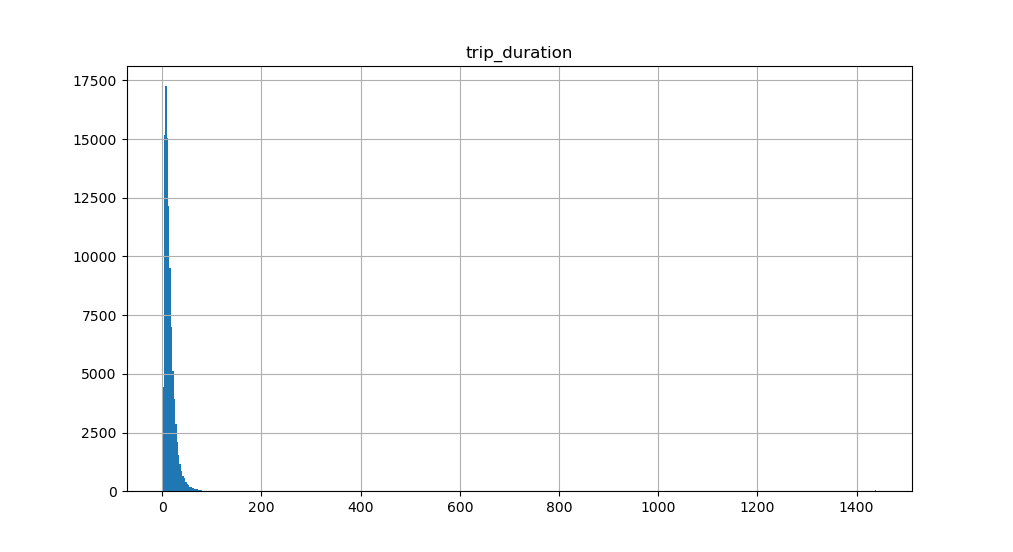
\includegraphics[width=\linewidth]{hist_duration_all}
  \caption{Histogram of all trip durations in minutes.}
  \label{fig:hist_dur_all}
\end{figure}

\begin{figure}[h]
  \centering
  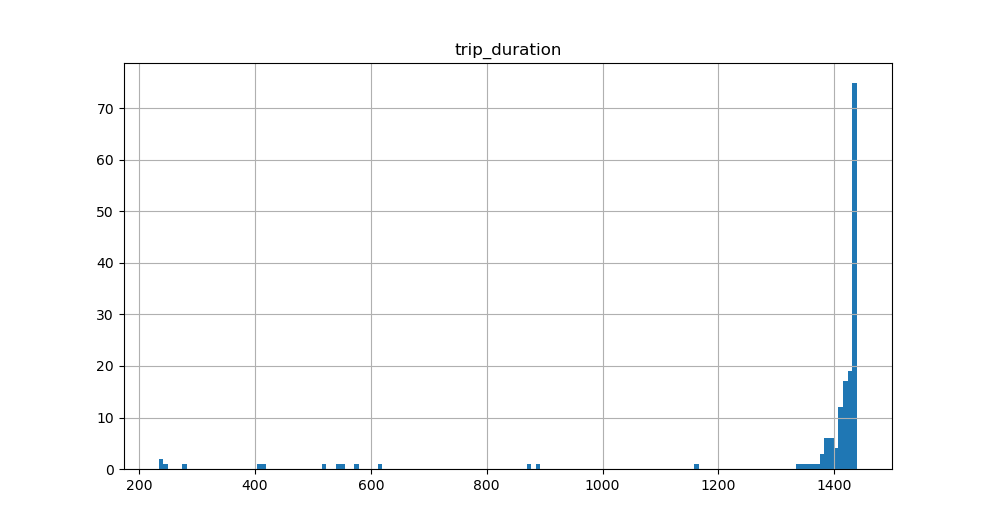
\includegraphics[width=\linewidth]{hist_duration_outliers}
  \caption{Histogram of all trip durations longer than 200 minutes.}
  \label{fig:hist_dur_out}
\end{figure}

Next, the ratio of trip durations to trip distances was calculated to get the average time in minutes that was needed per mile for every taxi trip. Figure ~\ref{fig:hist_durdist_out} shows the values for taxi rides that need more than 75 minutes per mile. It can be seen that not many trips are included in this plot, so we set the threshold to 100 minutes per mile and data tuples exceeding this value were filtered. The resulting histogram of the average minutes needed per mile is displayed in Figure ~\ref{fig:hist_durdist_filt}. In order to analyze and visualize this metric more easily, the values below or equal to 20 minutes per mile were binned into nine intervals. We chose the tenth interval to contain all values greater than 20 minutes per mile because this can be seen as an upper bound for most data points according to Figure ~\ref{fig:hist_durdist_filt}. 

\begin{figure}[h]
  \centering
  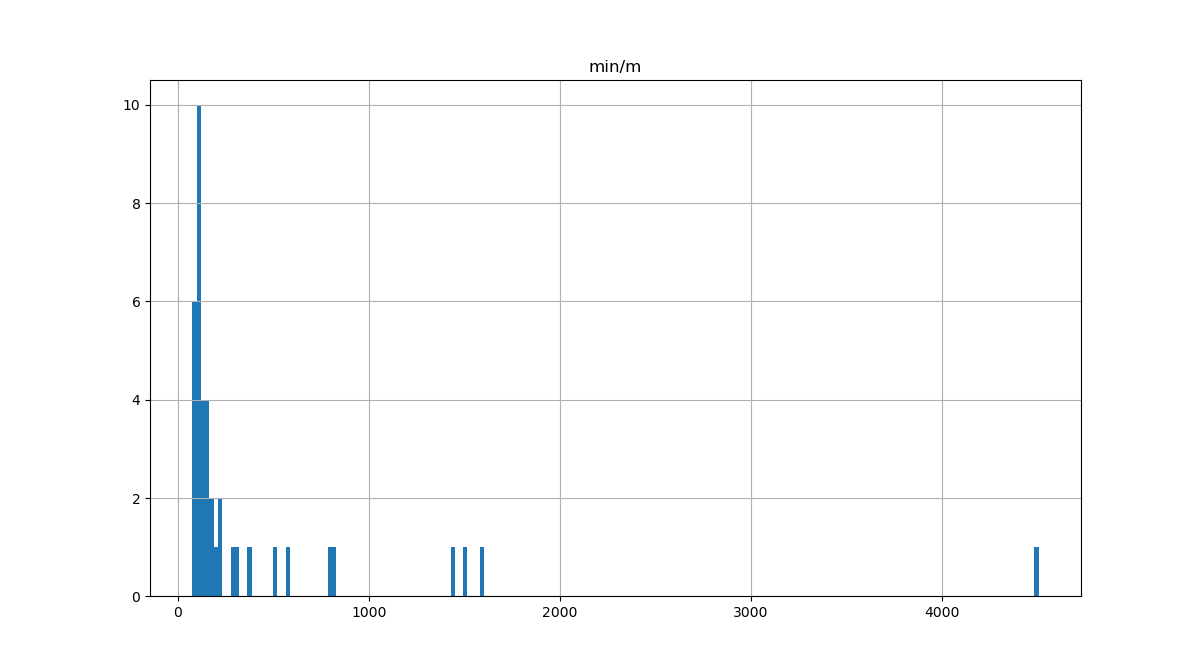
\includegraphics[width=\linewidth]{hist_durtodist_outliers}
  \caption{Histogram of the ratio between trip duration and trip distance in minutes per mile. Only ratios greater than 75 minutes per mile are shown}
  \label{fig:hist_durdist_out}
\end{figure}

\begin{figure}[h]
  \centering
  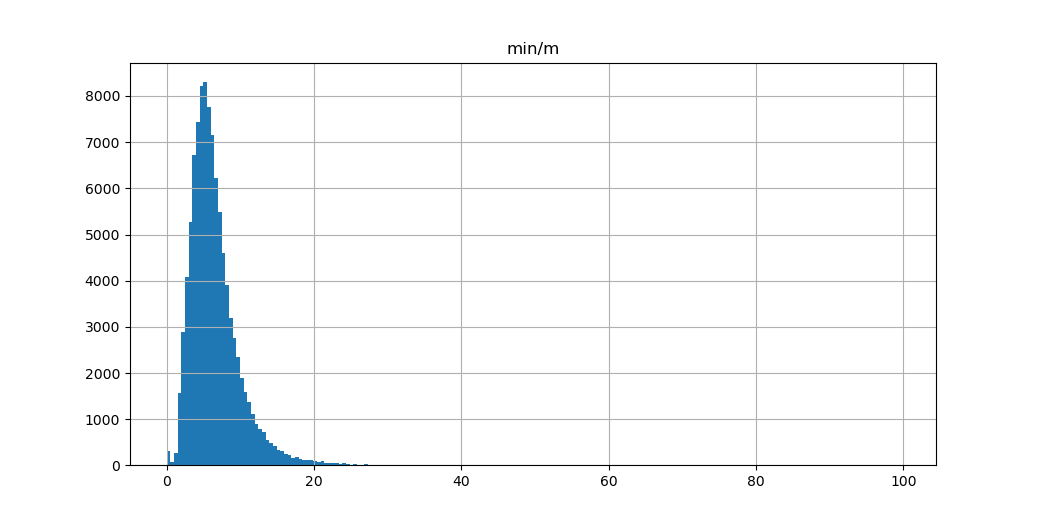
\includegraphics[width=\linewidth]{hist_durtodist_filtered}
  \caption{Histogram of the ratio between trip duration and trip distance in minutes per mile for the filtered data set.}
  \label{fig:hist_durdist_filt}
\end{figure}


Another metric we calculated was the ratio of the trip distances to the fare amounts. This can be understood as the price in Dollar the passengers had to pay per mile and is beneficial in the visualization process as high fare amounts on short trips indicate interesting outliers within the dataset.\\
The ratio can easily be calculated by dividing the fare amount by the trip distance, however, we decided to deduct the initial fare ride of $2.5\$$ for each trip as this amount is to be paid regardless of the trip distance ~\citep{fareamount}. In order to maintain a reasonable range, we decided to limit this metric between 0 and 40 Dollars per mile.



To distinguish trips taken on workdays against weekends, we calculated the corresponding weekday from the date for each ride.\\


Finally, after performing the preprocessing steps, the resulting data set consists of 101.315 entries and is saved as a CSV file. This file is then used for the clustering algorithm that is explained in the next section.




\section{Application}
\label{sec:app}

Since we decided to visualize the data using \textit{Kepler.gl}, we rely on React as our application interface. React works with the use of components, thus the map has to be instantiated as such.\\
Loading the data can be done with the provided \textit{Processors} module, however, the CSV file requires to be converted into a JavaScript module. We do this by performing the clustering algorithm on the CSV file in a Python script and exporting the resulting data set as a string. Note that ''export default'' needs to be prepended.\\

Once the map component is mounted, the data can be displayed with the \textit{addDataToMap} function according to a specified configuration which defines how the data is displayed. 
Point, Line, Polygon, Heatmap or Icon are some of the possible shapes with which the data can be encoded in a layer. Layers can be filtered by the data attributes to only display the desired range. Visual variables such as size and color can further be encoded by attributes.
The final configuration we used can be found in the file \textit{src/components/global.js}.\\

Another JavaScript file defines the general look of the application. Besides small changes regarding the logo and title, we furthermore modified the sidebars. Since the user should only be able to explore the data and not delete it or change the visualizations, we removed the left sidebar provided by \textit{kepler.gl}. Instead, we implemented a sidebar on the right side that gives deeper information about the data and is introduced in Section ~\ref{sec:tripdetail}. Furthermore, unnecessary functions as switching to a 3D map or a dual map view were removed.



\subsection{Clustering}
\label{sec:cluster}

As we aim to analyze the geographic context information contained in the data set, our first goal is to identify New York City's hotspots from the taxi data. Hotspots are defined as the most frequented places in the city, so a clustering algorithm suits best to find these places. We apply the Density-based spatial clustering of applications with noise (DBSCAN) because it finds clusters with points that are close together, marks other points as outliers and does not need a predefined, fixed number of clusters. Pickup, as well as drop-off locations, are equally selected as input to the algorithm. Hyperparameters were found by using trial and error. The parameter specifying the minimum density is set to $\epsilon = 0.001$ and the minimum number of points for a cluster $minPts$ is calculated with Formula ~\ref{formula:minPts}. 

\begin{align}
\label{formula:minPts}
minPts = 0.003 \cdot len(data)
\end{align}

The DBSCAN algorithm is implemented in Python and applied to the whole data set to find general hotspots, but also to a data set containing only taxi trips on weekdays and one containing only trips on weekends. With this separated computation, the geographic context can be analyzed regarding differences in the time of the week. For the whole data set 12 clusters are found, while for weekdays and weekends we get 16 clusters each. \\
When starting the application, the user sees the clusters obtained from the whole data set. Different colors of the data points show which cluster they belong to. Outliers, so points that are not part of a cluster, are colored cyan and displayed much smaller than the other points to be separable from them. On the right side of the application, it is possible to switch between the three different clusterings. After hovering over the map, the application updates to the chosen view. Accordingly, one can select one of the clusters to get more detailed information about it. On the one hand, the view is changed to display only the chosen cluster and zoomed in to the threshold value described in Section ~\ref{sec:zoom}, where the data points' visual variables are different. Moreover, when the user zooms out, lines appear that connect the drop-offs inside the cluster with the respective pickup location. The lines are colored according to the cluster the pickup belongs to. The restriction of showing only drop-off locations is due to the limitations of the Kepler tool and further explained in Section ~\ref{sec:challenges}. On the other hand, the information the trip details offer is adapted to this specific cluster. These analyses are explained in Section ~\ref{sec:tripdetail}.






\subsection{Points of Interest}
\label{sec:poi}

Once the data is spatially clustered as described in the previous section, we aim to visually explain the context behind these different clusters. Our initial assumption states that places such as tourist attractions, sports venues as well as other hubs of public transportation such as train stations and airports are causing heavy traffic on taxis in New York City.\\ 
To verify these claims we visualize points of interest for each cluster. Several APIs for retrieving geospatial information about companies or landmarks were at our disposal, namely Yelp, Foursquare and Google Places. Our first approach utilizes the Yelp interface, where the results are heavily biased toward restaurants. While some of those are possible and likely candidates for generating clusters, none of our initial assumed places are contained in the results. Foursquare provides similarly unpleasant results which is why we utilize the Nearby Search of Google Places API \footnote{https://developers.google.com/places/web-service/search (24.03.2020)} for our final result.\\
For each of our clusters, we first calculate the geographical center and use these coordinates to request places within a radius of 300m from Google. These results are ranked by prominence, meaning their importance towards Google. However, we discover when ranking the results by the number of user ratings, the more popular places are found amongst the top results. We use the top 10 results of each cluster and visualize these locations on the map with a blue pin. Examples are given in Section ~\ref{sec:analysis}, where the points of interest are used to confirm the presence of clusters and explain differences of frequency between weekdays and weekends.




\subsection{Semantic Zoom}
\label{sec:zoom}

To take advantage of the large space the Powerwall offers, semantic zooming is implemented to be able to display different levels of detail. In general, the size of the data points depends on the current zooming level and is calculated using Formula ~\ref{formula:zoom}, where the variable $newR$ represents the new radius of the data point.

\begin{align}
\label{formula:zoom}
newR = ((currentZ - minZ) \cdot R) + maxR\\
R = \dfrac{minR - maxR}{maxZ - minZ}
\end{align}\\

After experimenting with different settings on the Powerwall, following parameters were defined: minimum radius $minR=0.5$, maximum radius $maxR = 19.37$, minimum zoom level $minZ = 10$, and maximum zoom level $maxZ = 19$. $CurrentZ$ is the value of the current zoom level. We made sure that the radius of data points never gets below the minimum radius value so that the data points can still be perceived.\\ 
Accordingly, a threshold of $thrZ = 15.9$ was set to specify the zoom level where the view of the application changes. When this zoom level is reached, the data points' shape, color and size are modified and depend on different attributes from the data set.\\
First, the shape of the data points displays the type of location. We use different icons to represent the type of data point, namely an arrow for pickup locations and a ring for drop-off locations. The color now represents the trip duration in relation to the trip distance, so the average time needed per mile. Using the bins from the data preprocessing explained in Section ~\ref{sec:data}, a color scale from white to red is created and fitted to the different bins. The more red a data point is colored, the more minutes are needed per mile for this taxi trip. By choosing the color scale like this, outliers are easily detectable and can be examined further. A third change affects the size of the data points. The size now depends on the average dollar paid per mile. The more the passengers had to pay for a mile, the bigger the data point gets. Besides this, the size still changes according to the zoom level as described in the beginning. Only variable $minZ$ needs to be adapted to $minZ = 16$ for the icons.
 Some interesting patterns and striking taxi rides can be seen, which is exemplarily shown in Section ~\ref{sec:analysis}. \\
This view is also triggered when the user selects a specific cluster, which is explained in Section ~\ref{sec:cluster}. Zooming out effects the displayed view insofar that the data points of the cluster are drawn as points again. Because of the limitations of the Kepler tool described in Section ~\ref{sec:challenges}, unfortunately, only drop-off locations can be displayed. These drop-offs are connected to the respective pickup location with a line in the color of the pickup's cluster. All in all, three different levels of granularity are obtained by the implementation of semantic zooming: a general overview, connections between clusters and a detailed view of individual clusters. Figure ~\ref{fig:semanticzoom} gives an example of all three possible views.



\begin{figure}[!htb]
\minipage{0.32\linewidth}
  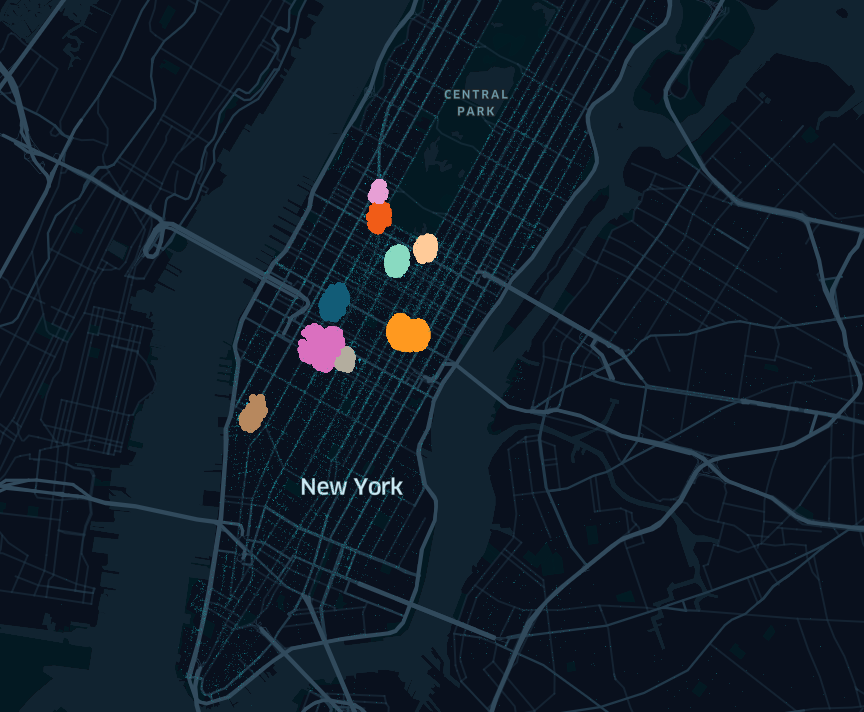
\includegraphics[width=\linewidth]{semanticzoom1}
\endminipage\hfill
\minipage{0.32\linewidth}
  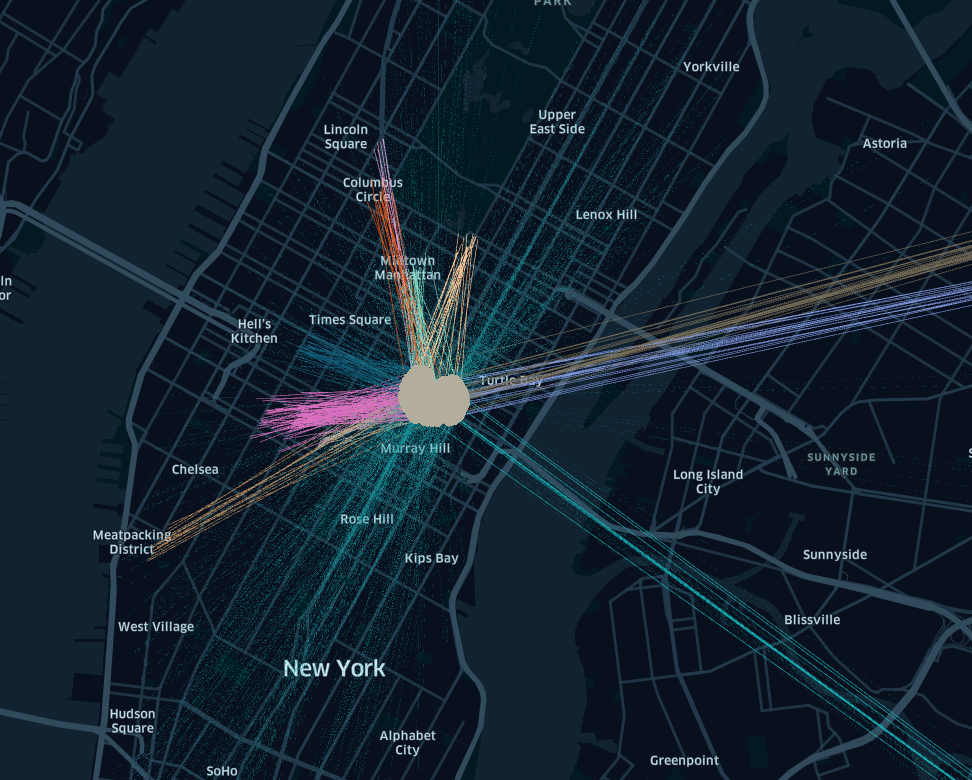
\includegraphics[width=\linewidth]{semanticzoom2}
\endminipage\hfill
\minipage{0.32\linewidth}%
  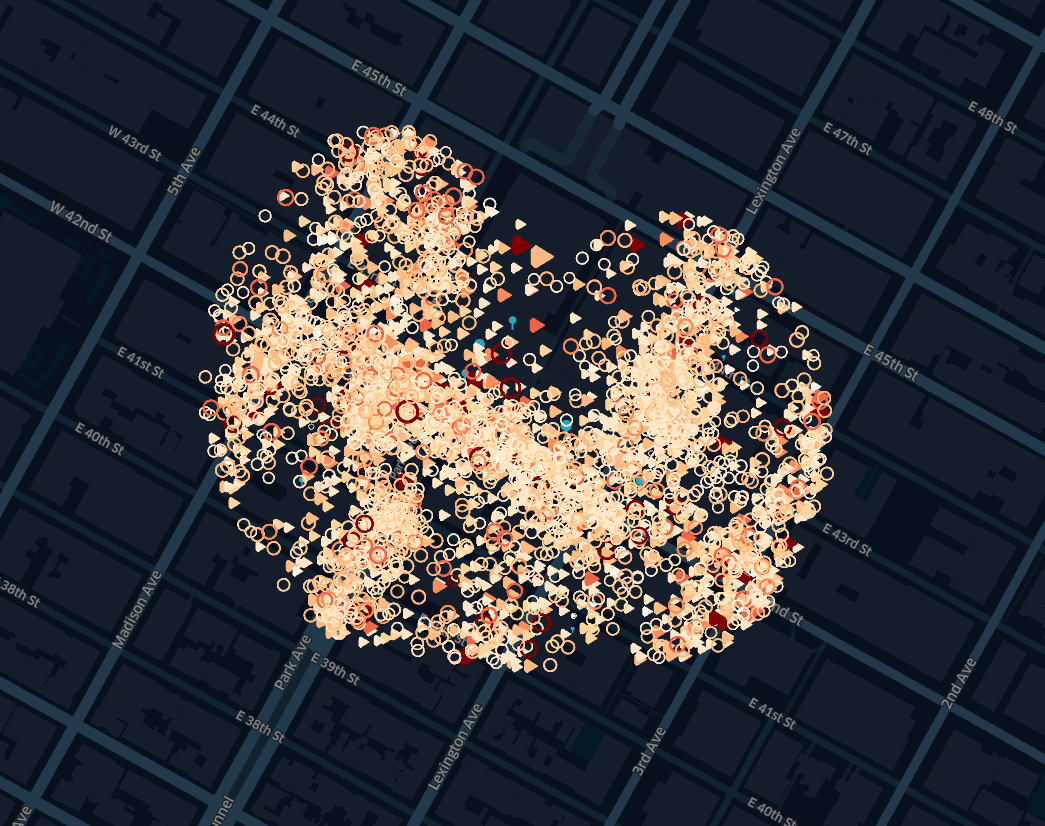
\includegraphics[width=\linewidth]{semanticzoom3}
\endminipage
\caption{Example showing the three different levels of granularity realized by semantic zooming.}
\label{fig:semanticzoom}
\end{figure}





\subsection{Trip Details}
\label{sec:tripdetail}

In contrast to visualizing each data point on the map, we want to further investigate the data on a broader scope. To achieve this, we implemented a side view to give insights about the data attributes using different plots, as shown in Figure ~\ref{fig:sideplots}.\\
To visualize the frequency of trips in relation to their temporal aspect over a day, we realize a clock glyph with a cyan and orange line representing the pickup and drop-off frequency respectively. The cyan colored area behind these lines indicates the frequencies across the entire dataset.\\

The passenger count attribute has a range from 1 to 6 in discrete steps, which is why we decided on a bar chart for visualization. Again, one specific cluster can be discriminated against the entire dataset, as the orange bar describes all available data and the cyan bar restricts to the data of the cluster. \\
As the trip distance and fare amount are continuous attributes, a density plot seemed the most appropriate to highlight the most frequent data range.\\

Furthermore, this section of the screen provides interactivity to the tool as different data can be selected. A selection between the entire dataset, only workdays, or only weekends can be made, where different clusters will be shown regarding the selection. A specific cluster can be examined closer by choosing it from the dropdown button. Once a cluster is selected, the view of the map will center on this cluster and the points of interest for this cluster will be displayed on the side. Moreover, the plots will now compare the data from the cluster against the entire data set.



\begin{figure}[h]
  \centering
  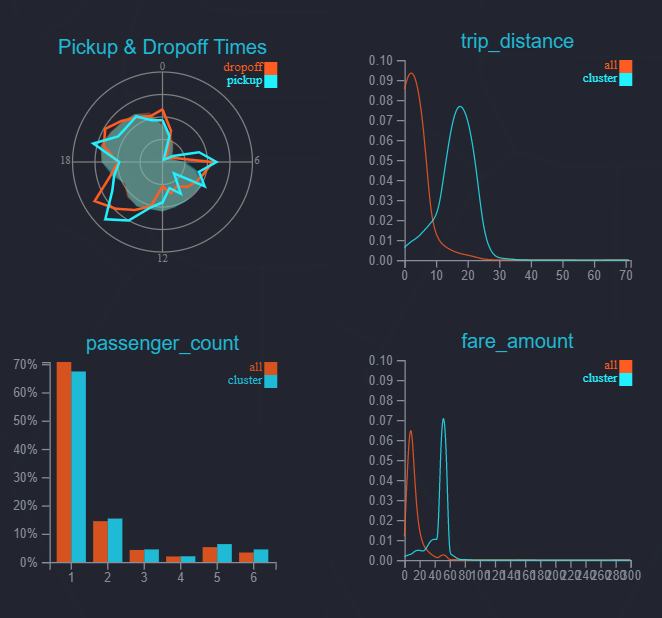
\includegraphics[width=0.95\linewidth]{sideplots}
  \caption{Aggregated view of the plots describing the entire dataset in comparison to a specific cluster.}
  \label{fig:sideplots}
\end{figure}






\section{Evaluation}
\label{sec:analysis}

In this section, specific analyses are presented that confirm the usefulness of our application. Visual data exploration is performed to obtain deeper knowledge about the underlying data.\\
Regarding the location of hotspots in New York City, the comparison between weekdays and weekends gives interesting information. Figure ~\ref{fig:clusters_day} shows the clusters obtained from the data set containing only taxi trips on weekdays. In contrast to the overview of weekends shown in Figure ~\ref{fig:clusters_end}, cluster 16 seems to appear only on weekdays. Having a closer look at cluster 16, like in Figure ~\ref{fig:cluster16_day}, the trip details give valuable information about this cluster. The points of interest in this area represent, almost exclusively, doctors. This fits the different pickup and drop-off times from the average times and explains why this cluster is only present on weekdays and not on weekends.


\begin{figure}[h]
  \centering
  \begin{subfigure}[b]{0.95\linewidth}
	  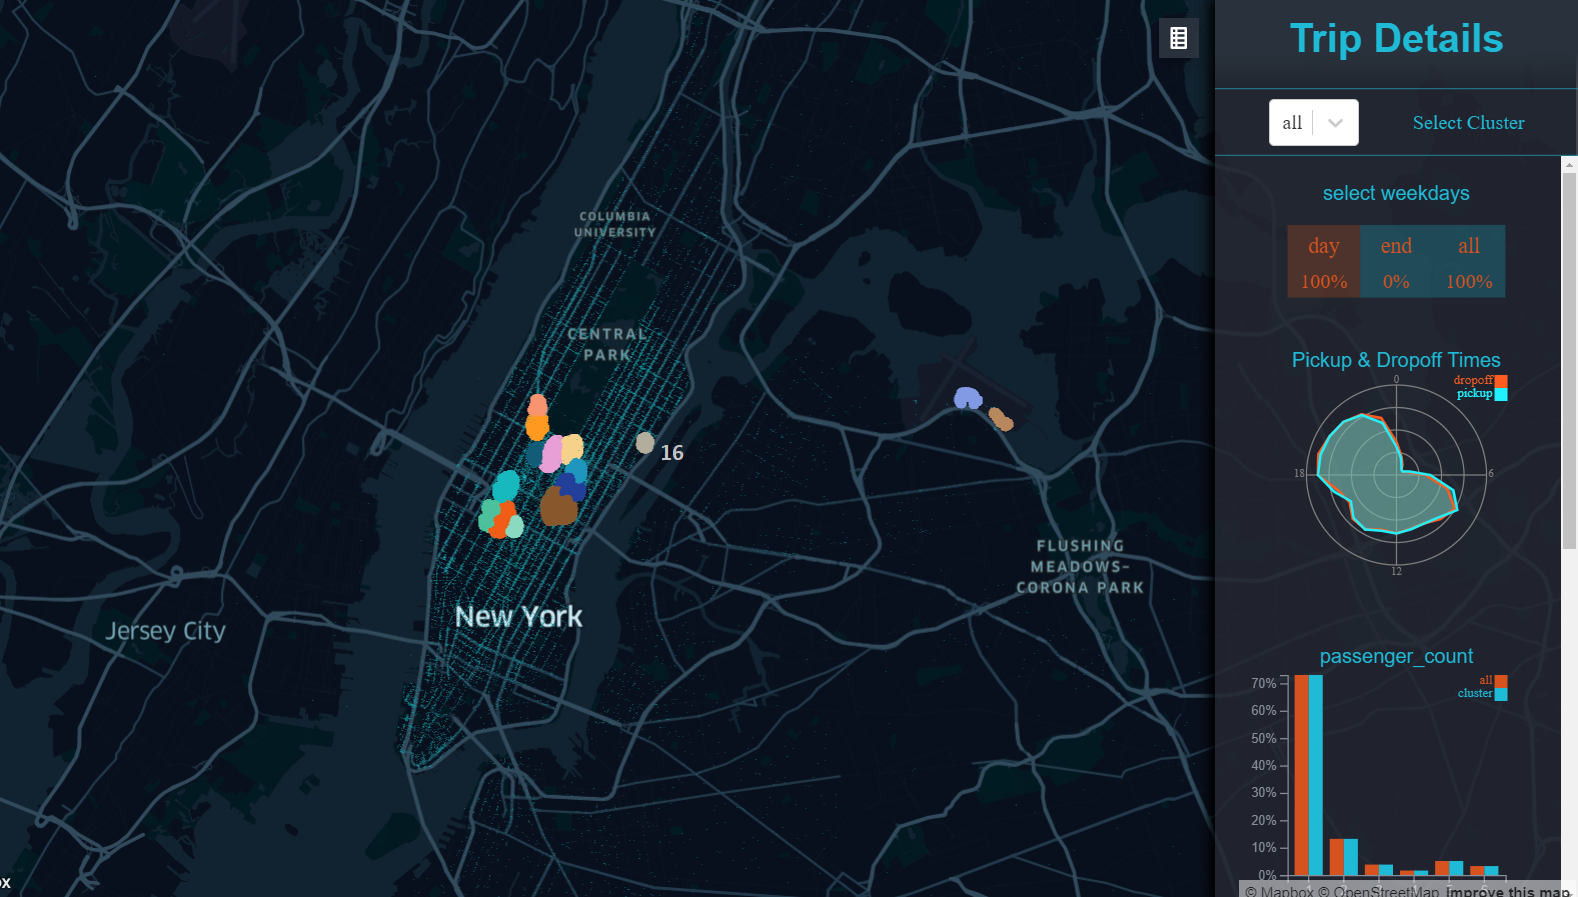
\includegraphics[width=\linewidth]{clusters_day}
  	  \caption{}
  	  \label{fig:clusters_day}
  \end{subfigure}
  
  \begin{subfigure}[b]{0.95\linewidth}
	  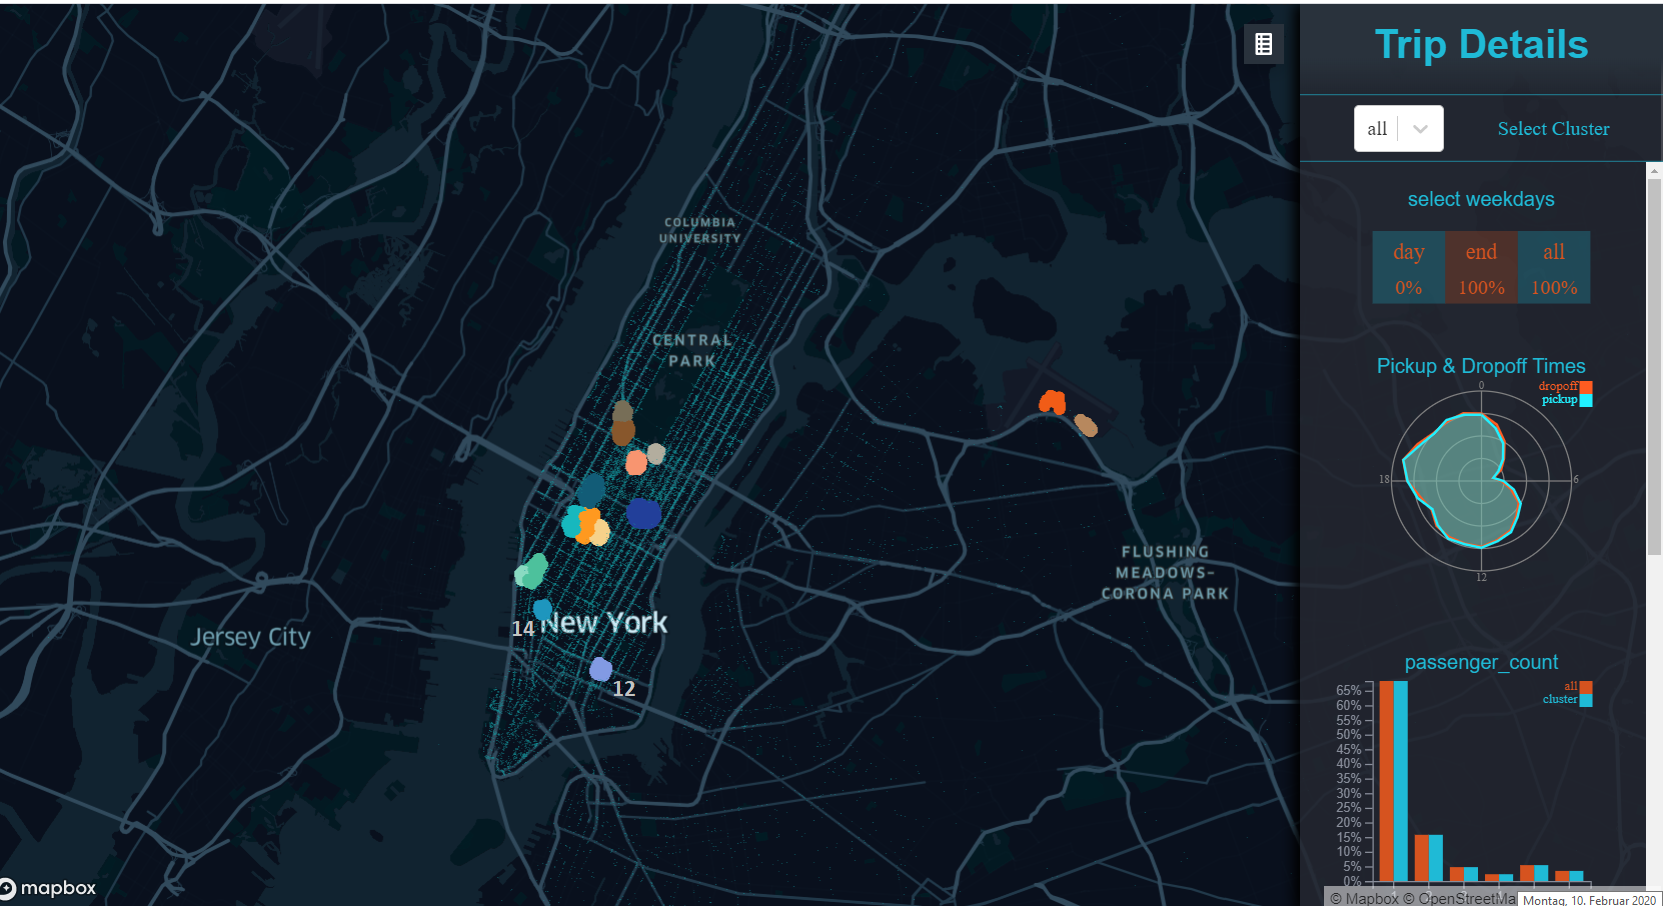
\includegraphics[width=\linewidth]{clusters_end}
	  \caption{}
	  \label{fig:clusters_end}
  \end{subfigure}
\caption{Two overviews of all located clusters from the DBSCAN algorithm. (a) Clusters from weekday data. (b) Clusters from weekend data.}
\end{figure}

\begin{figure}[h]
  \centering
  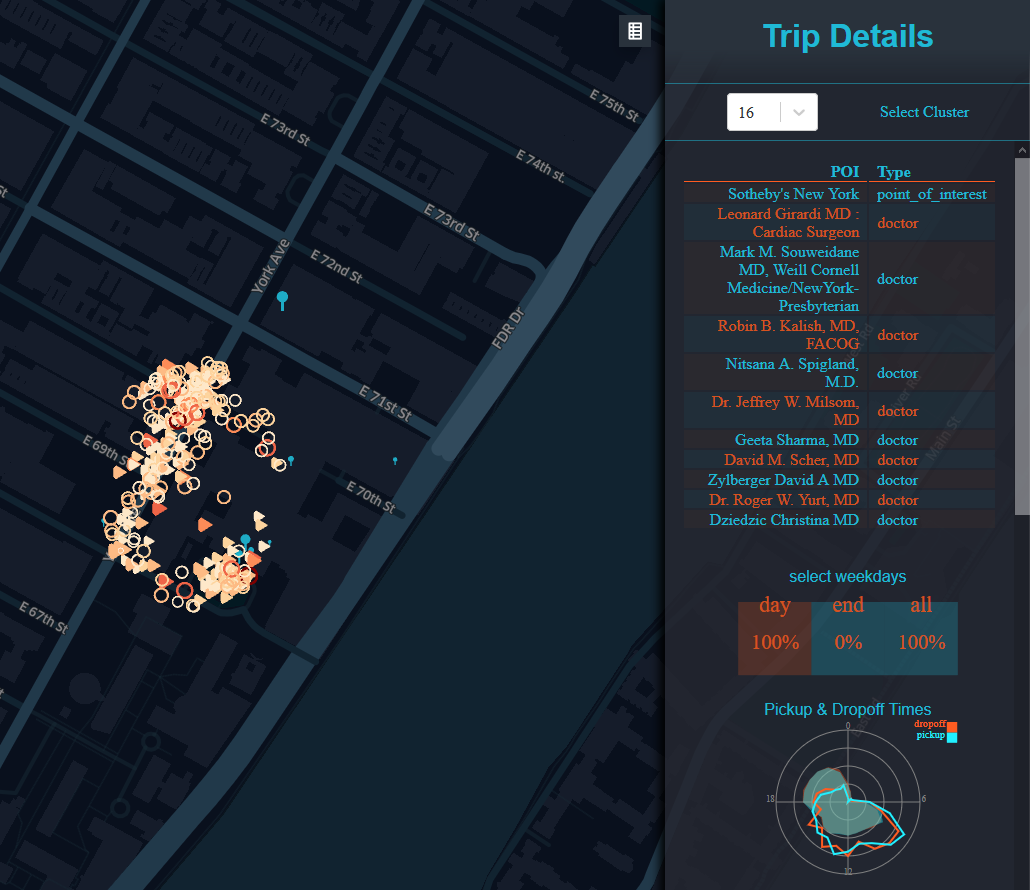
\includegraphics[width=0.95\linewidth]{cluster16_day}
  \caption{Zoomed in cluster 16 from the weekday data.}
  \label{fig:cluster16_day}
\end{figure}

Accordingly, looking at clusters 12 and 14 of the weekend data that are not present on weekdays, it is noticeable that especially bars and night clubs are located there. \\

The two relationships between trip distance and trip duration and between trip distance and fare amount that are visible when the view is zoomed in can be compared. In doing so, it is possible to detect outliers and see if both measures are consistent. Small and light data points indicate taxi trips with a reasonable duration and fare amount for the distance covered. Red and small data points show taxi rides that took longer than expected, but with a price that is still legitimate. An example in the left picture of Figure ~\ref{fig:outliers} shows a taxi ride that was 1.3 miles long, took over 26 minutes and cost 16 Dollars. On the contrary, light and large data points display taxi trips with a valid duration but a very high fare amount. These represent mostly very unusual taxi rides of a very short distance. In the middle picture, you can see an example of a ride that was 0.3 miles long, lasted 7 seconds but had a fare amount of 52 Dollars. Finally, in the last picture, a taxi ride is displayed that shows abnormal values for both metrics. While the distance is very short with only 0.2 miles, the trip lasted over 15 minutes and cost 10 Dollars. Interestingly, the two airport clusters do not contain many outliers. Since they are located outside of the city center, this confirms that there is much traffic inside the city and the outliers result probably because of that.\\
By visually exploring the data points and relationships, abnormal data values can be perceived. They either represent special taxi rides and striking features of the data or are the result of unclean data. Unfortunately, without an expert, it is hard to discriminate between both possibilities. However, using our application these data points can be identified easily and fast and help to analyze the data.





\begin{figure}[!htb]
\minipage{0.32\linewidth}
  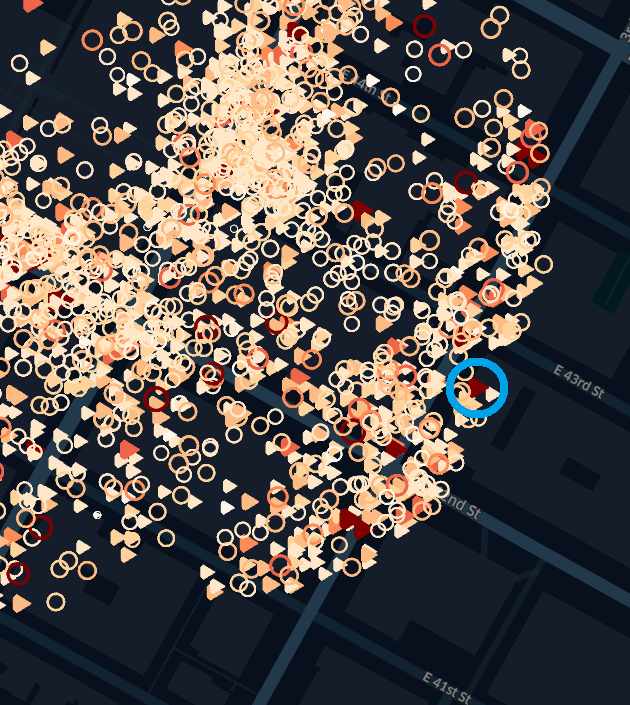
\includegraphics[width=\linewidth]{outlier_time}
\endminipage\hfill
\minipage{0.32\linewidth}
  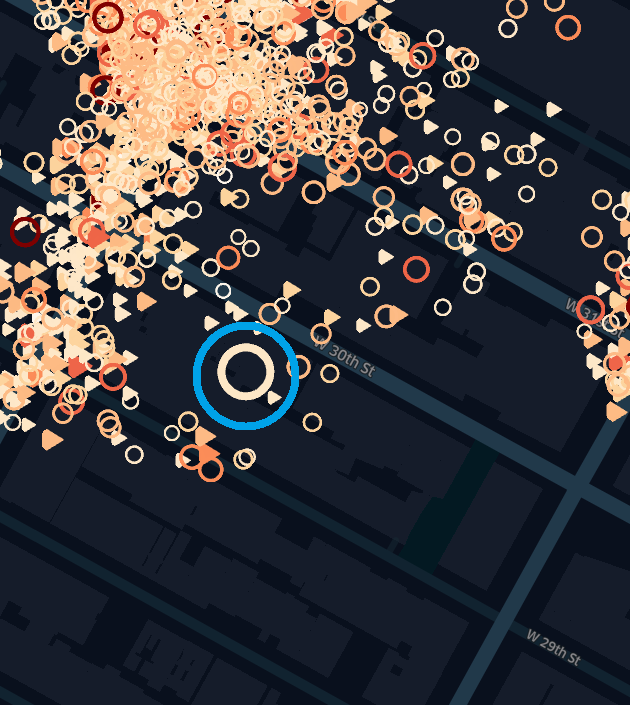
\includegraphics[width=\linewidth]{outlier_fare}
\endminipage\hfill
\minipage{0.32\linewidth}%
  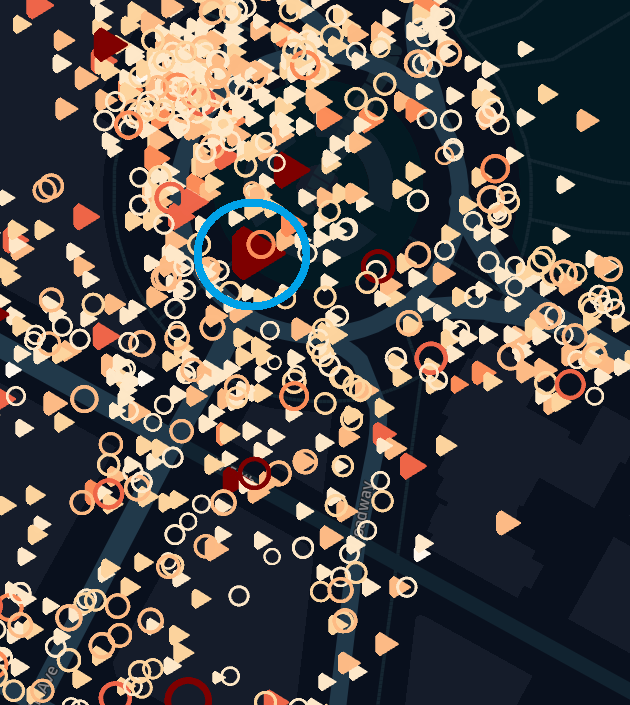
\includegraphics[width=\linewidth]{outlier_both}
\endminipage
\caption{Examples of special data points and outliers. The blue circle shows the respective data point.}
\label{fig:outliers}
\end{figure}


The implemented trip details provide information to compare single clusters with the entire data set and find out more about taxi rides starting and ending in this area. One outstanding cluster represents the area of an airport. Since the airport is located outside the city center, it is not surprising that the trip distance and fare amount are considerably higher than average for this cluster. Pickup and drop-off times are more often at noon than in the evening compared to other taxi rides. This could correlate with flights usually taking place at these times. \\
Cluster 10 shows significantly many taxi trips around 7 ~pm and 11 ~pm, as can be seen in Figure ~\ref{fig:cluster10_times}. The points of interest in this area include, inter alia, the Lincoln Center for the Performing Arts and the Metropolitan Opera House. It could be that events start and end at these times and cause the two peaks in the clock glyph. 

\begin{figure}[h]
  \centering
  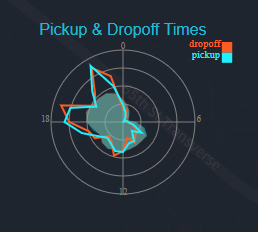
\includegraphics[width=0.4\linewidth]{cluster10_times}
  \caption{Pickup and drop-off times of cluster 10.}
  \label{fig:cluster10_times}
\end{figure}

Accordingly, cluster 14 of the weekend data set that was already mentioned at the beginning of this section, shows interesting trip details. Since it consists almost exclusively of bars, pickup and drop-off times are mostly in the late evening and the night as expected. Furthermore, the bar plot for passenger counts shows fewer rides with only one passenger, but more rides with two or more passengers. This seems reasonable, as most people do not go out alone but with friends.\\
This way, all clusters can be further examined and interesting facts can be found out. 




\section{Challenges and Limitations}
\label{sec:challenges}

In this section, we discuss the challenges we faced during the development of our application. Furthermore, limitations of the underlying \textit{Kepler.gl} tool are presented that restrict the implementation of additional features.\\
One big problem we had to deal with is the limited amount of data that can be pre-loaded into \textit{Kepler.gl}. By saving the data set as a text file as described in Section ~\ref{sec:app}, we manage to pre-load a data set of about 100.000 entries. Unfortunately, this is less data than for one month. Of course, we would get more profound analyses and findings when we integrate more data into our calculations. Furthermore, temporal influences over longer periods are not identifiable. When starting the project, we set up a database to manage all taxi trip data and be able to incorporate additional data. As soon as we realized that we cannot process a big amount of data, we decided to work without a database as this additional step was not necessary anymore. Accordingly, the weather data we collected ~\footnote{https://www.ncdc.noaa.gov/ (26.11.2019)} that should provide further context information is currently not used in the application. Now we concentrate only on the taxi data that can be processed and loaded into the tool and try to get as much knowledge out of it as possible. In a first version of the application, subway stations of New York City were also shown on the map. Since they did not provide deeper information about the data set, we decided not to include them.\\


As already mentioned in Section ~\ref{sec:cluster} and ~\ref{sec:zoom}, we are only able to display drop-off locations when the user selects a cluster and zooms out. This problem occurs because of the way filters are implemented in \textit{Kepler.gl}. There is a limitation of one filter per data set, so it is not possible to filter the cluster of drop-offs and pickups together. Because of this, we only zoom in when a cluster is selected to be able to show all data points belonging to the cluster. When zooming out, we change the view to display the connections between clusters and show where people come from. To visualize only relevant taxi trips for the chosen cluster with lines from pickup to drop-off location, we need to apply a filter to the data set. Since we want to show where people come from and are only able to apply one filter, we decided to select only the drop-offs of the specified cluster. This is the reason why pickup locations are not visible anymore in this view. One possibility to overcome this limitation would be to define a variable that contains both pickup and drop-off cluster and filter according to this attribute. The problem, in this case, is that you need to specify all possible occurrences of this variable by hand. Arrays are treated as strings in the Kepler tool and therefore not suitable to implement the filter efficiently. For 16 clusters, we would need to cover $16^2 = 256$ possible values of the variable and develop a method to select all relevant data points where either pickup or drop-off cluster is equal to the selected one. Another option would be to load the data set twice into the application and apply the filter for the pickup cluster to one data set and the filter for the drop-off cluster to the other data set. In doing so, we could see all relevant data points for a chosen cluster easily. Unfortunately, as described before, only a limited number of data points can be pre-loaded into the Kepler tool. For this reason, we do not want to slow it down or limit the data even more by loading two big data sets. Furthermore, we would need to adapt all other implementations to two data sets, so we decided not to try this option. Browsing through open issues for the Kepler tool, we notice that filtering is one topic that is currently worked on and maybe with a newer version of the application it is possible to apply multiple filters to a data set ~\citep{openissues}.\\

Another limitation caused by \textit{Kepler.gl} relates to the possible visualizations of data points. The shape of a data point can only be a classical point or one of some pre-defined icons. Icons include symbols like a cross or an arrow but also figures like a car, a clock, a basketball and many more. As far as we know, it is not possible to define customized shapes. Moreover, only the radius and the color of data points can easily be adapted according to an attribute of the data. For example, it is possible to define the color according to the cluster the data point is assigned to. In contrast, other visual characteristics like the opacity or outlines cannot be changed in this way and need a fixed value. These properties of \textit{Kepler.gl} make it hard to dynamically change the visualization of data points when the user zooms in or out. It is not feasible to integrate more data attributes by modifying more visual variables.\\

Finally, there are some drawbacks concerning the general appearance of the application and the visualizations. Despite the implementation of semantic zooming, there is still some occlusion of data points visible that makes the map unclear to some extent. We thought about to not only increase the size of the data points when zooming out but to cluster neighboring data points and make the visualization more simple. Unfortunately, we did not have enough time to try an aggregation in \textit{Kepler.gl}. Furthermore, hovering works not well in the application. When the user moves the mouse over a data point, a tooltip pops up that gives more detailed information about this specific data point. In the current version, it is sometimes not possible to get the information of the tooltip for the desired data point, since it is hard to select.\\

Summarizing the challenges we faced during the development of our application, note that most problems are due to the limitations of the \textit{Kepler.gl} itself. It is not possible to modify everything the way we want it to be and we have to stick to the basic structure. 







\section{Outlook}
\label{sec:outlook}

In this section, we present future work that can be done to improve our application to make it more useful or applicable to other tasks.\\
To refer to some problems mentioned in Section ~\ref{sec:challenges}, one big upgrade would be to integrate more data. On the one hand, we could confirm our present results and refine the analyses. On the other hand, some interesting patterns that are not obvious depend on external factors, like the weather, public holidays or events. It would be nice to analyze the geographic context more detailed and detect peculiarities in the data.\\
This can also be realized by providing more information about the clusters, for example by integrating the opening times for the points of interest.\\


As seen in Section ~\ref{sec:analysis}, many interesting clusters and anomalies are due to temporal influences. Our attempt to visualize the time of day for each data point failed since \textit{kepler.gl} does not offer many possibilities to modify the data points and using different colors turned out to be very unclear. Therefore, an idea would be to perform the clustering not only for weekdays and weekends, but also for different times of day, for example, morning, noon, evening, and night. This would provide the user with additional information about the differences between taxi rides concerning various time points and facilitate the comparison of clusters.\\
Related to this suggestion is the implementation of comparing two clusters directly. By now, it is only possible to compare a cluster to the entire data set, but not to a different cluster. \\




Another possible extension relates to the duration and fare amount of taxi rides. When we have enough data, we can make predictions about a taxi trip given the start and end location as well as the time when it should happen. By analyzing all available taxi rides, it is possible to compute the probable duration of the hypothetical taxi ride together with the fare amount. This could help passengers to plan their trips and decide when to go by taxi.\\
Moreover, this tool could be of interest for taxi companies. Having the information about frequent locations and times, this helps to determine where taxis have to be stationed and make it more efficient.\\

Concerning the Powerwall, extensions to give even more detailed views of the data points would be interesting. Since we have this large space and good resolution available, it could be exploited more effectively with better visualizations. However, the mentioned limitations of \textit{kepler.gl} make it very hard to modify the data points more and develop more comprehensive views. 




\section{Conclusion}
\label{sec:conclusion}

In this paper, we present the development of an application for the Powerwall to perform geographic context analyses of the New York Taxi Data set. The application is based on the \textit{kepler.gl} tool and provides visualizations in three different levels of detail. Using the Powerwall offers great opportunities for semantic zooming and showing overviews as well as a more detailed view of the data. Hotspots of New York City are identified by a clustering of the data points. Additional analyses of the data set are shown in a sidebar and compare pickup with drop-offs as well as single clusters with the entire data set. By performing exemplary evaluations, the usefulness of the application is shown. Especially the good resolution of the Powerwall contributes to a clear and useful visualization that can be further examined. Finally, we discuss the limitations of the implemented tool and show how it can be extended for future use cases.







%%
%% The next two lines define the bibliography style to be used, and
%% the bibliography file.
\bibliographystyle{ACM-Reference-Format}
\bibliography{literature}

%%
%% If your work has an appendix, this is the place to put it.
%\appendix
%\section{Research Methods}
%\subsection{Part One}



\end{document}
\endinput
